% A0 portrait conference poster - a0poster + multicols.
%
%   pdflatex poster.tex        (run twice)
%
% Needs alongside it: fig_pipeline.png, fig_scaling.png, qr_repo.png
%
% Design follows Faulkes (Better Posters), Carter (Designing Science
% Presentations) and the Argonne poster guide: three columns, 64 mm margins,
% prose rather than bullets, no boxes or rules around sections, three colours,
% one sans-serif family, title set as a conclusion rather than a topic.
%
% TUNING, in the order to try it: reduce \figbandwidth, then \bodysize. Do not
% reduce the margins - roughly 30% of the sheet should stay white.

\documentclass[a0,portrait,final]{a0poster}

\usepackage[left=64mm,right=64mm,top=55mm,bottom=45mm]{geometry}
\usepackage{multicol}
\usepackage[utf8]{inputenc}
\usepackage[T1]{fontenc}
\usepackage{helvet}
\renewcommand{\familydefault}{\sfdefault}
\usepackage{xcolor}
\usepackage{graphicx}
\usepackage{amsmath}
\usepackage{tikz}
\usetikzlibrary{positioning,arrows.meta}

% ---------------------------------------------------------------- palette ---
\definecolor{cq}{HTML}{2A78D6}      % quantum / built surface / headings
\definecolor{cc}{HTML}{EB6834}      % classical / vegetation
\definecolor{ca}{HTML}{1BAF7A}      % third series
\definecolor{ink}{HTML}{0B0B0B}
\definecolor{ink2}{HTML}{52514E}
\definecolor{muted}{HTML}{8A8A85}
\definecolor{surface}{HTML}{FCFCFB}
\pagecolor{surface}
\color{ink}

% ----------------------------------------------------------- layout knobs ---
\newcommand{\ttlsize}{\fontsize{100}{112}\selectfont}
\newcommand{\subsize}{\fontsize{44}{54}\selectfont}
\newcommand{\authsize}{\fontsize{40}{50}\selectfont}
\newcommand{\headsize}{\fontsize{48}{58}\selectfont}
\newcommand{\bodysize}{\fontsize{30}{40}\selectfont}
\newcommand{\capsize}{\fontsize{26}{34}\selectfont}
\newcommand{\blsize}{\fontsize{54}{66}\selectfont}
\newcommand{\finesize}{\fontsize{22}{28}\selectfont}

\newlength{\figbandwidth}
\setlength{\figbandwidth}{660mm}

\setlength{\columnsep}{64mm}
\setlength{\columnseprule}{0pt}   % white space separates columns, not a rule
\setlength{\parindent}{0pt}
\setlength{\parskip}{0pt}

% Section heading: coloured, never boxed, generous space above.
\newcommand{\shead}[1]{%
  \par\vspace{16mm}{\headsize\bfseries\color{cq}#1}\par\vspace{6mm}}
\newcommand{\sheadtop}[1]{%
  \par{\headsize\bfseries\color{cq}#1}\par\vspace{6mm}}
\newcommand{\figcap}[1]{\par\vspace{5mm}{\capsize\color{ink2}#1}\par}
\newcommand{\gap}{\par\vspace{7mm}}

\begin{document}
\sffamily

% ================================================================ title ====
\begin{minipage}{\textwidth}
{\ttlsize\bfseries
Quantum machine learning on satellite imagery:\\[6mm]
band selection, not qubit count, sets the cost\par}

\vspace{12mm}
{\subsize\color{ink2}
What a variational quantum classifier costs to run on multispectral data,
and which choice actually drives it\par}

\vspace{12mm}
{\authsize Deepesh V. Chaudhari\\[4mm]
{\color{ink2}National Geospatial-Intelligence Agency
\textperiodcentered{} 23 July 2026}\par}
\end{minipage}

\vspace{18mm}

% ====================================================== full-width figure ==
\begin{center}
  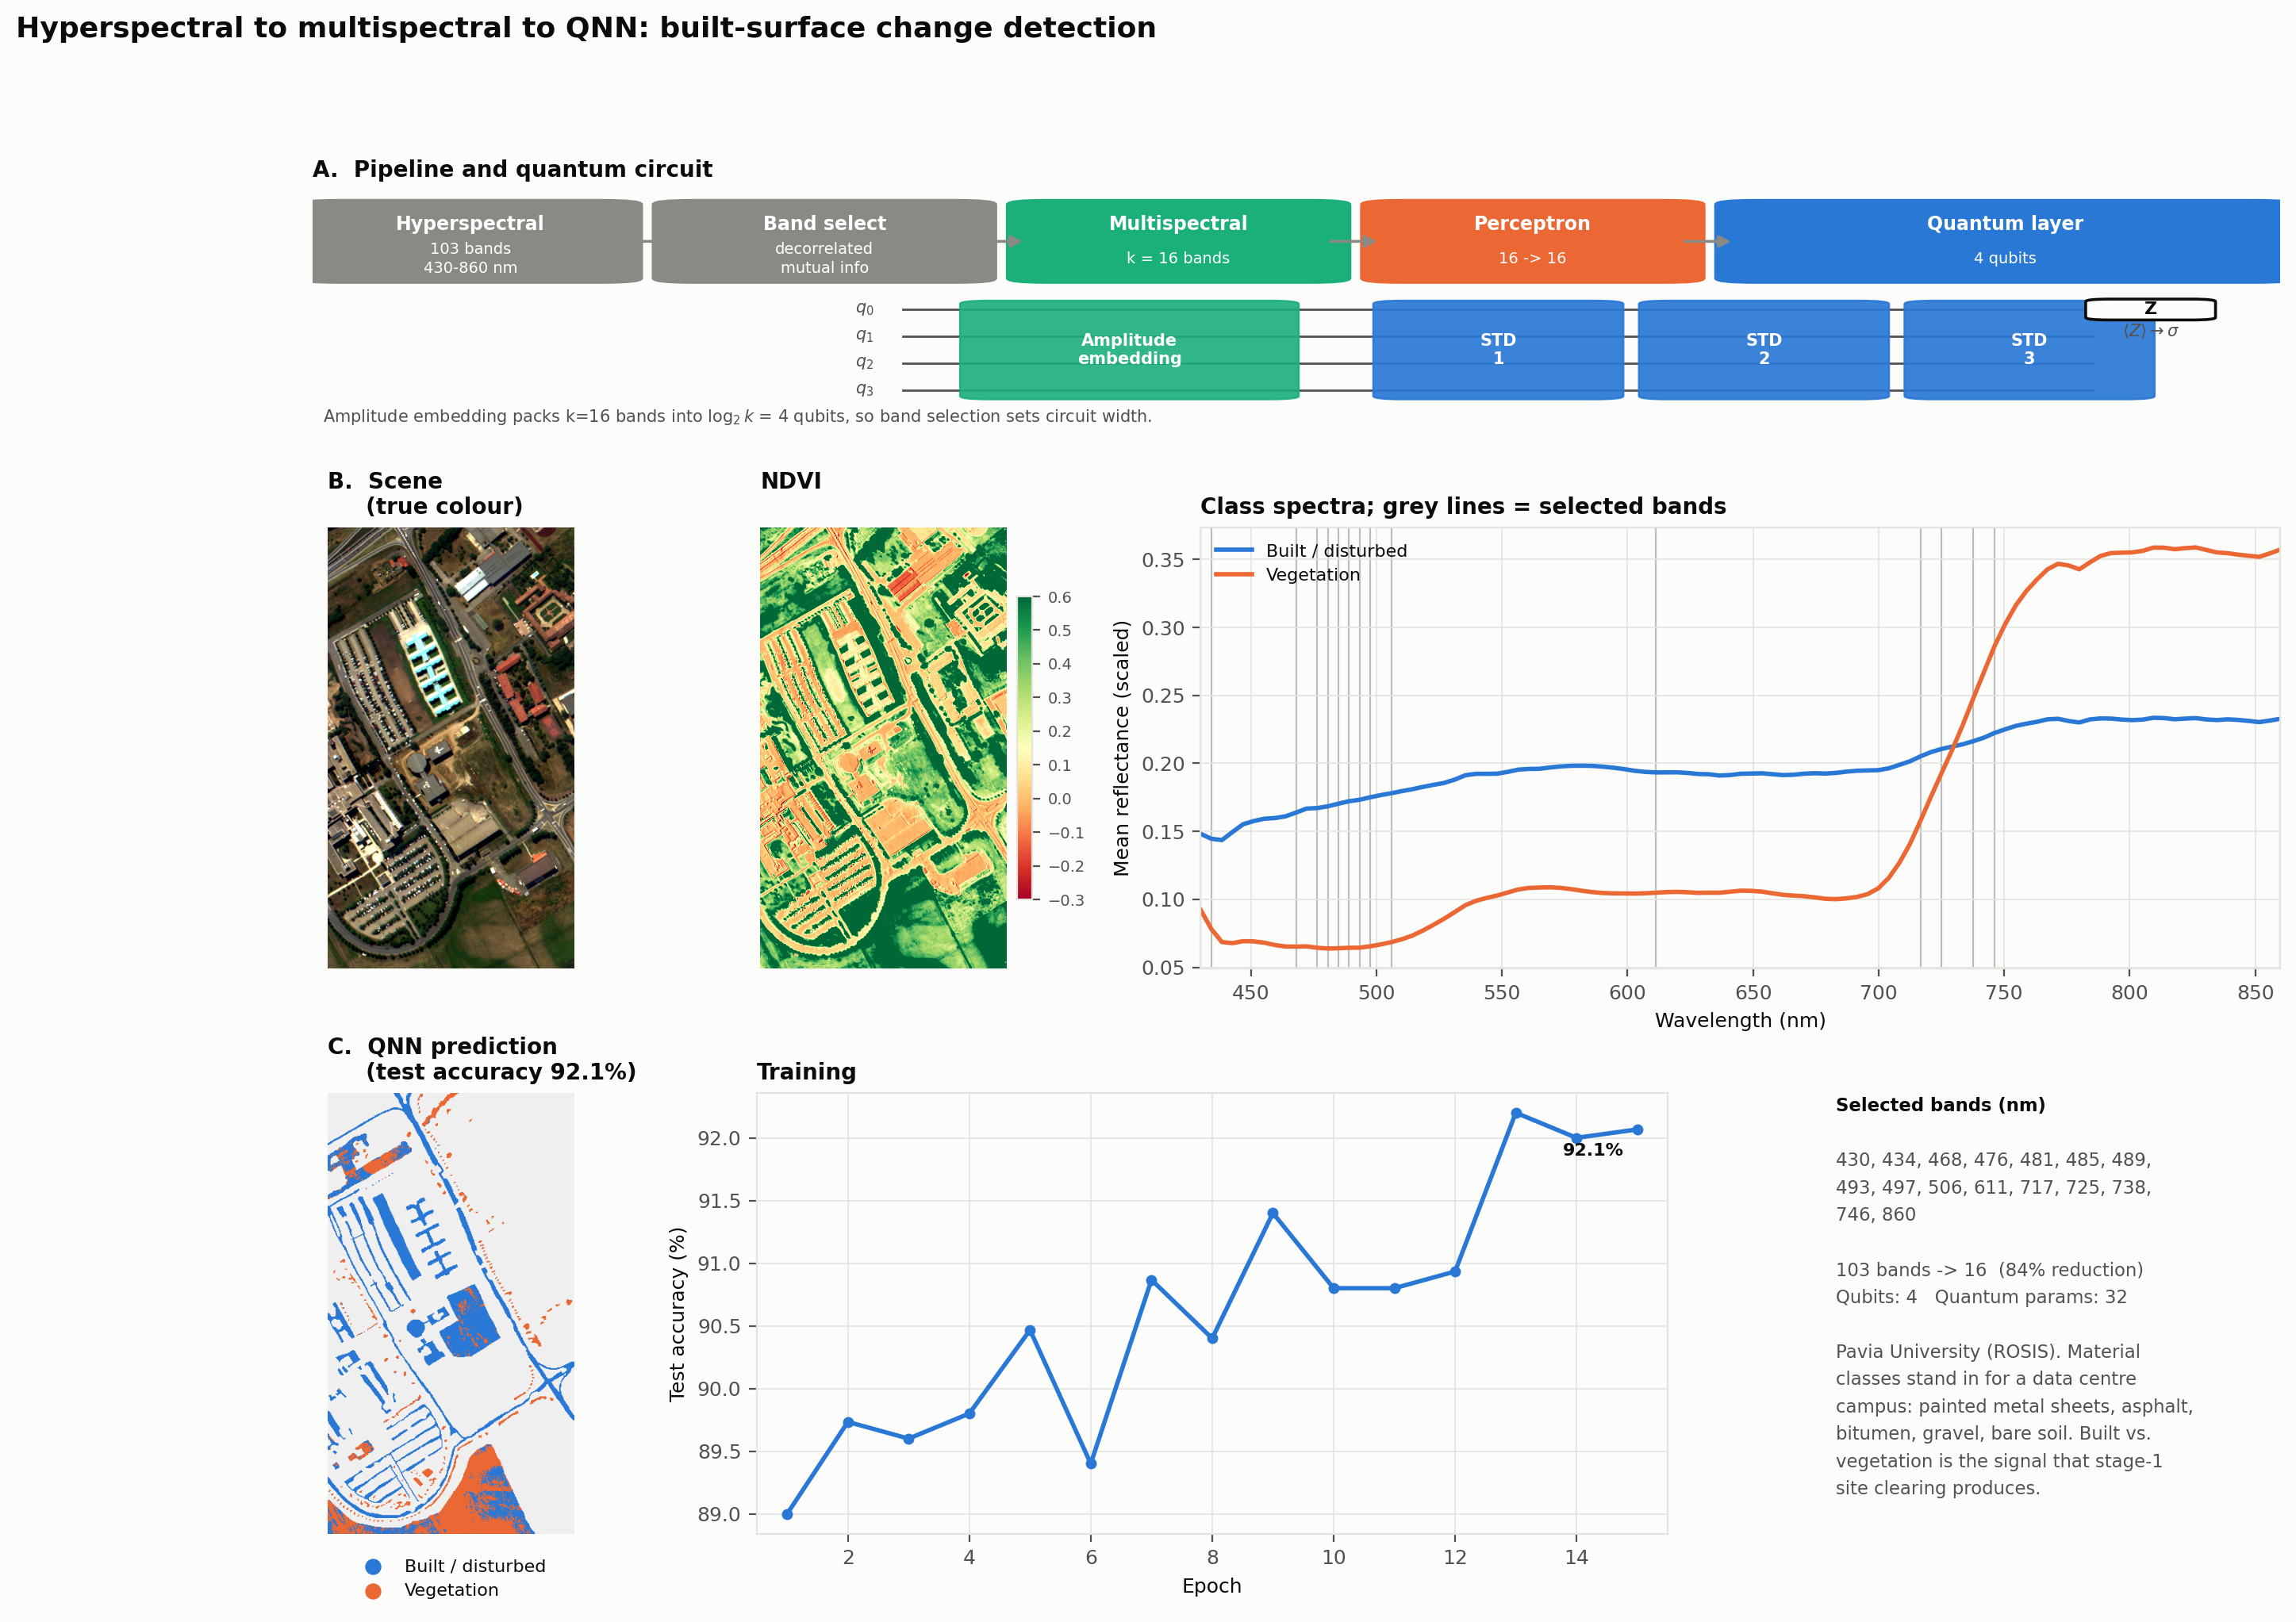
\includegraphics[width=\figbandwidth]{fig_pipeline.png}
\end{center}
\vspace{2mm}
{\capsize\color{ink2}
A 103-band hyperspectral cube is reduced by uniform band selection to a 16-band
multispectral stack, which feeds a hybrid model: a classical perceptron,
amplitude embedding, three SimplifiedTwoDesign layers, and a single-qubit
measurement. This is an independent implementation of the architecture described
in Rybotycki et al., not a run of their published code. The map shows a single
run at 94.7\%; the sweep in column two reports $95.2\pm0.3$\% across three
seeds.\par}

\vspace{18mm}

% ============================================================== columns ====
\begin{multicols}{3}
\raggedcolumns
\bodysize

%%% ------------------------------------------------------------- column 1 --
\sheadtop{Why anyone watches data centres}

Data centres are the physical substrate of AI capability~--- no frontier model
gets trained without one~--- and what companies announce about them routinely
diverges from what gets built. Case studies at Khazna's Ajman facility and xAI's
Memphis site both found gaps between public statements and observable
construction, and unpermitted equipment installed at Memphis was discovered from
overhead imagery, not from filings. Announcements, permits and press releases
cannot be relied on alone.
\gap
Imagery is the independent check. That makes tracking build-out a verification
problem~--- and verification across many sites and many revisits means
automation.

\shead{Which stages leave a signature}

Identifying the compute itself is not realistic~--- AI hardware shares halls
with general-purpose servers, carries no distinguishing visual signature, and
accounts for only 10--20\% of data centre power. What is tractable is detecting
change across repeat imagery.
\gap
Construction proceeds through eight stages. Six alter surface material in ways a
spectrometer registers: clearing strips vegetation, foundations expose concrete,
framing and roofing introduce metal, cladding changes it again, and cooling
plant adds structure. Planning and commissioning leave nothing to see.
\gap
That reduces to per-pixel classification, repeated over large scenes and many
revisits. The cost of that repetition is what this work measures.

\vspace{12mm}
% -- eight stages: fill only, no outlines --------------------------------
\begin{center}
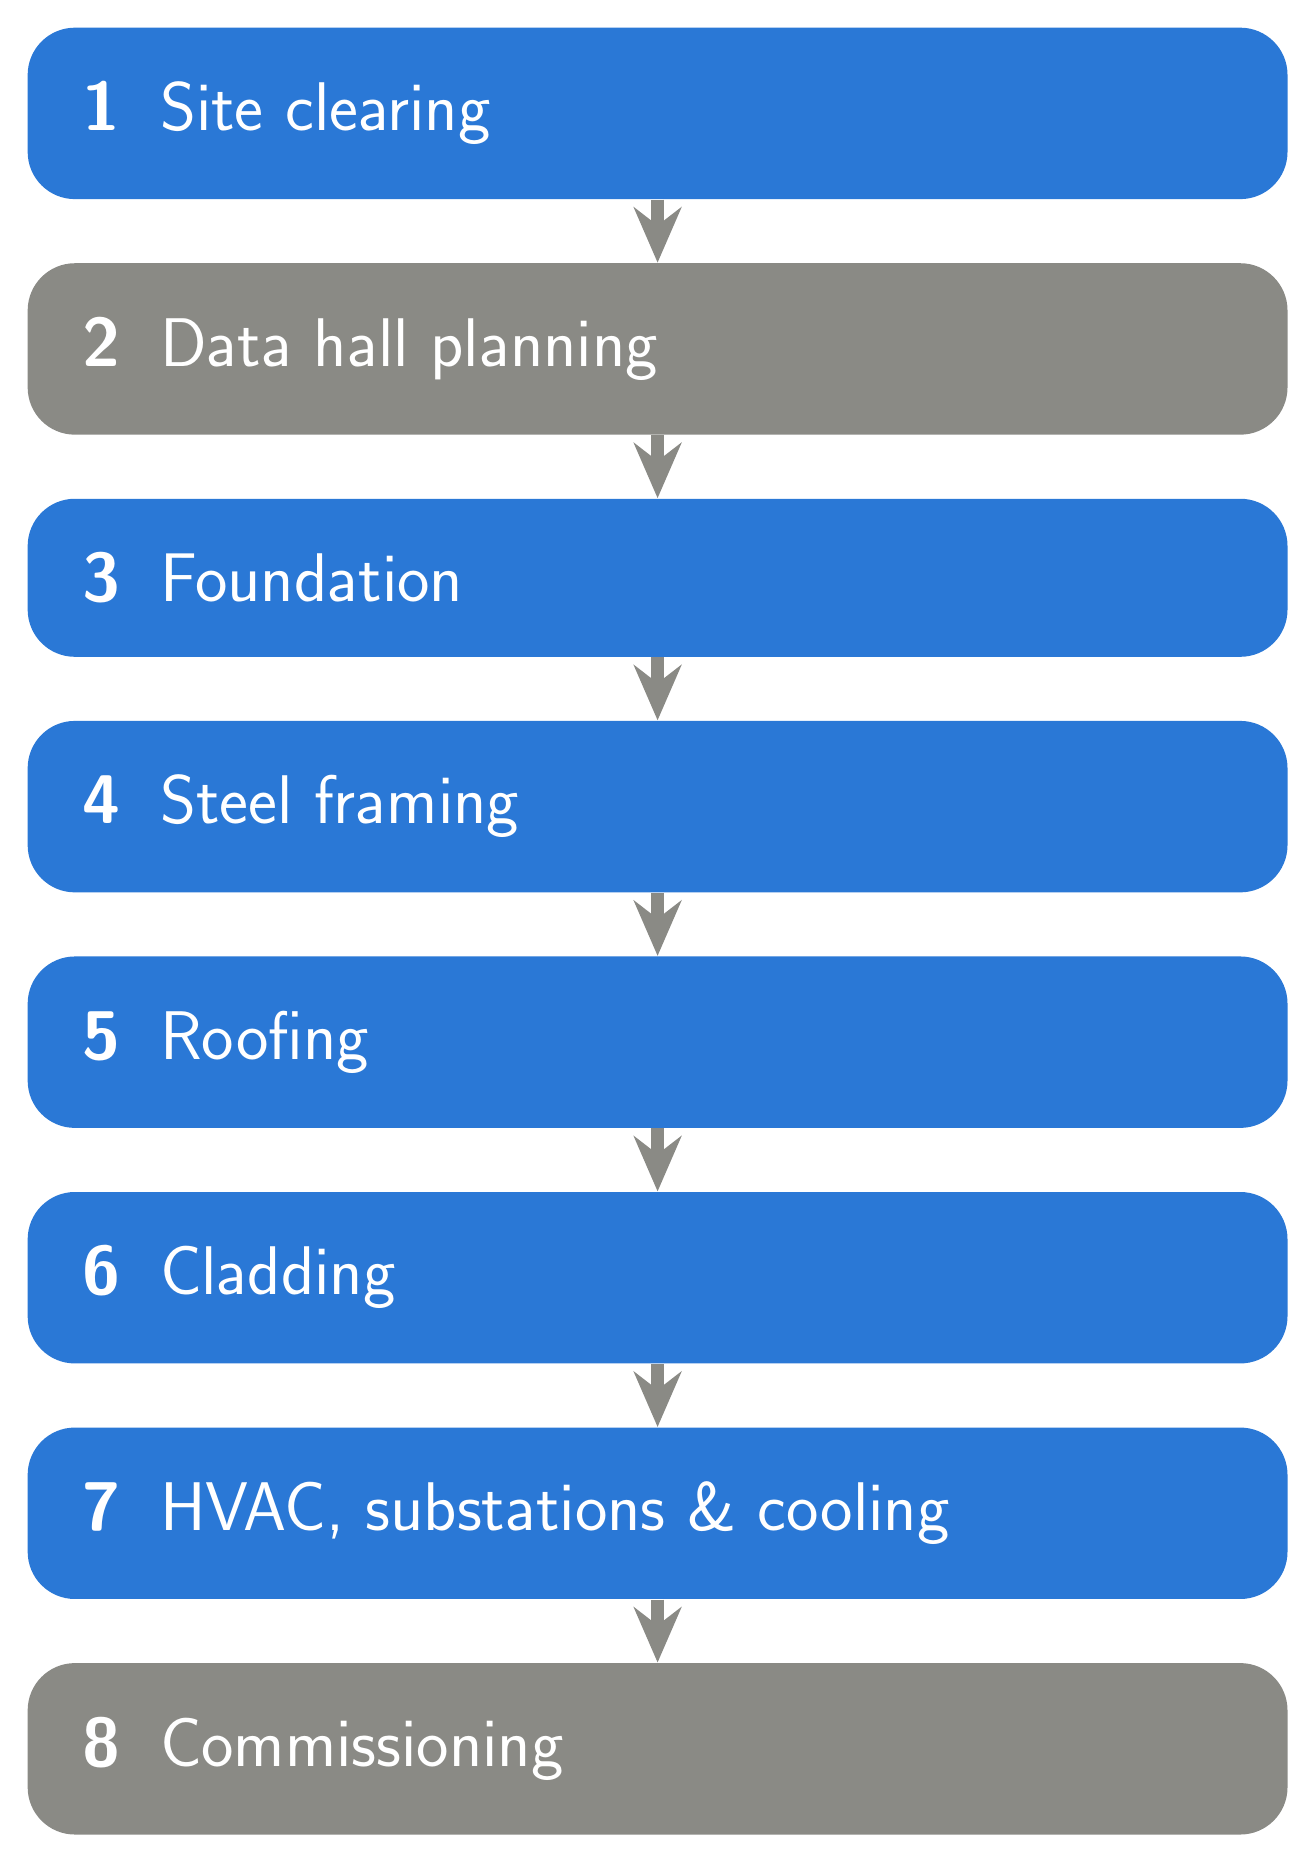
\begin{tikzpicture}[
  sb/.style={text width=146mm, align=left, rounded corners=6mm,
             inner sep=7mm, text=white,
             font=\fontsize{28}{34}\selectfont},
  arr/.style={-{Stealth[length=7mm,width=6mm]}, line width=1.6mm,
              color=muted}]
  \node[sb, fill=cq]                     (s1) {\textbf{1}\; Site clearing};
  \node[sb, fill=muted, below=8mm of s1] (s2) {\textbf{2}\; Data hall planning};
  \node[sb, fill=cq,    below=8mm of s2] (s3) {\textbf{3}\; Foundation};
  \node[sb, fill=cq,    below=8mm of s3] (s4) {\textbf{4}\; Steel framing};
  \node[sb, fill=cq,    below=8mm of s4] (s5) {\textbf{5}\; Roofing};
  \node[sb, fill=cq,    below=8mm of s5] (s6) {\textbf{6}\; Cladding};
  \node[sb, fill=cq,    below=8mm of s6] (s7) {\textbf{7}\; HVAC, substations
                                                  \& cooling};
  \node[sb, fill=muted, below=8mm of s7] (s8) {\textbf{8}\; Commissioning};
  \foreach \a/\b in {s1/s2,s2/s3,s3/s4,s4/s5,s5/s6,s6/s7,s7/s8}
    {\draw[arr] (\a) -- (\b);}
\end{tikzpicture}
\end{center}
\figcap{Six of eight stages leave a detectable spectral signature (blue);
planning and commissioning (grey) do not. Roofing and cladding are precisely
the painted-metal and bitumen classes this model separates.}

\columnbreak

%%% ------------------------------------------------------------- column 2 --
\sheadtop{A proxy, and why it holds}

Pavia University stands in for a data centre campus. No public hyperspectral
scene exists over a hyperscale facility, and this scene's material classes~---
painted metal sheets, asphalt, bitumen, gravel, bare soil~--- are what such a
campus is built from. Built-versus-vegetation is the signal that stage-one site
clearing produces.
\gap
Amplitude embedding packs $k$ bands into $\log_2 k$ qubits, so band selection
sets circuit width directly~--- a preprocessing choice that propagates into
hardware cost.

\shead{Accuracy plateaus, cost doubles}

\begin{center}
  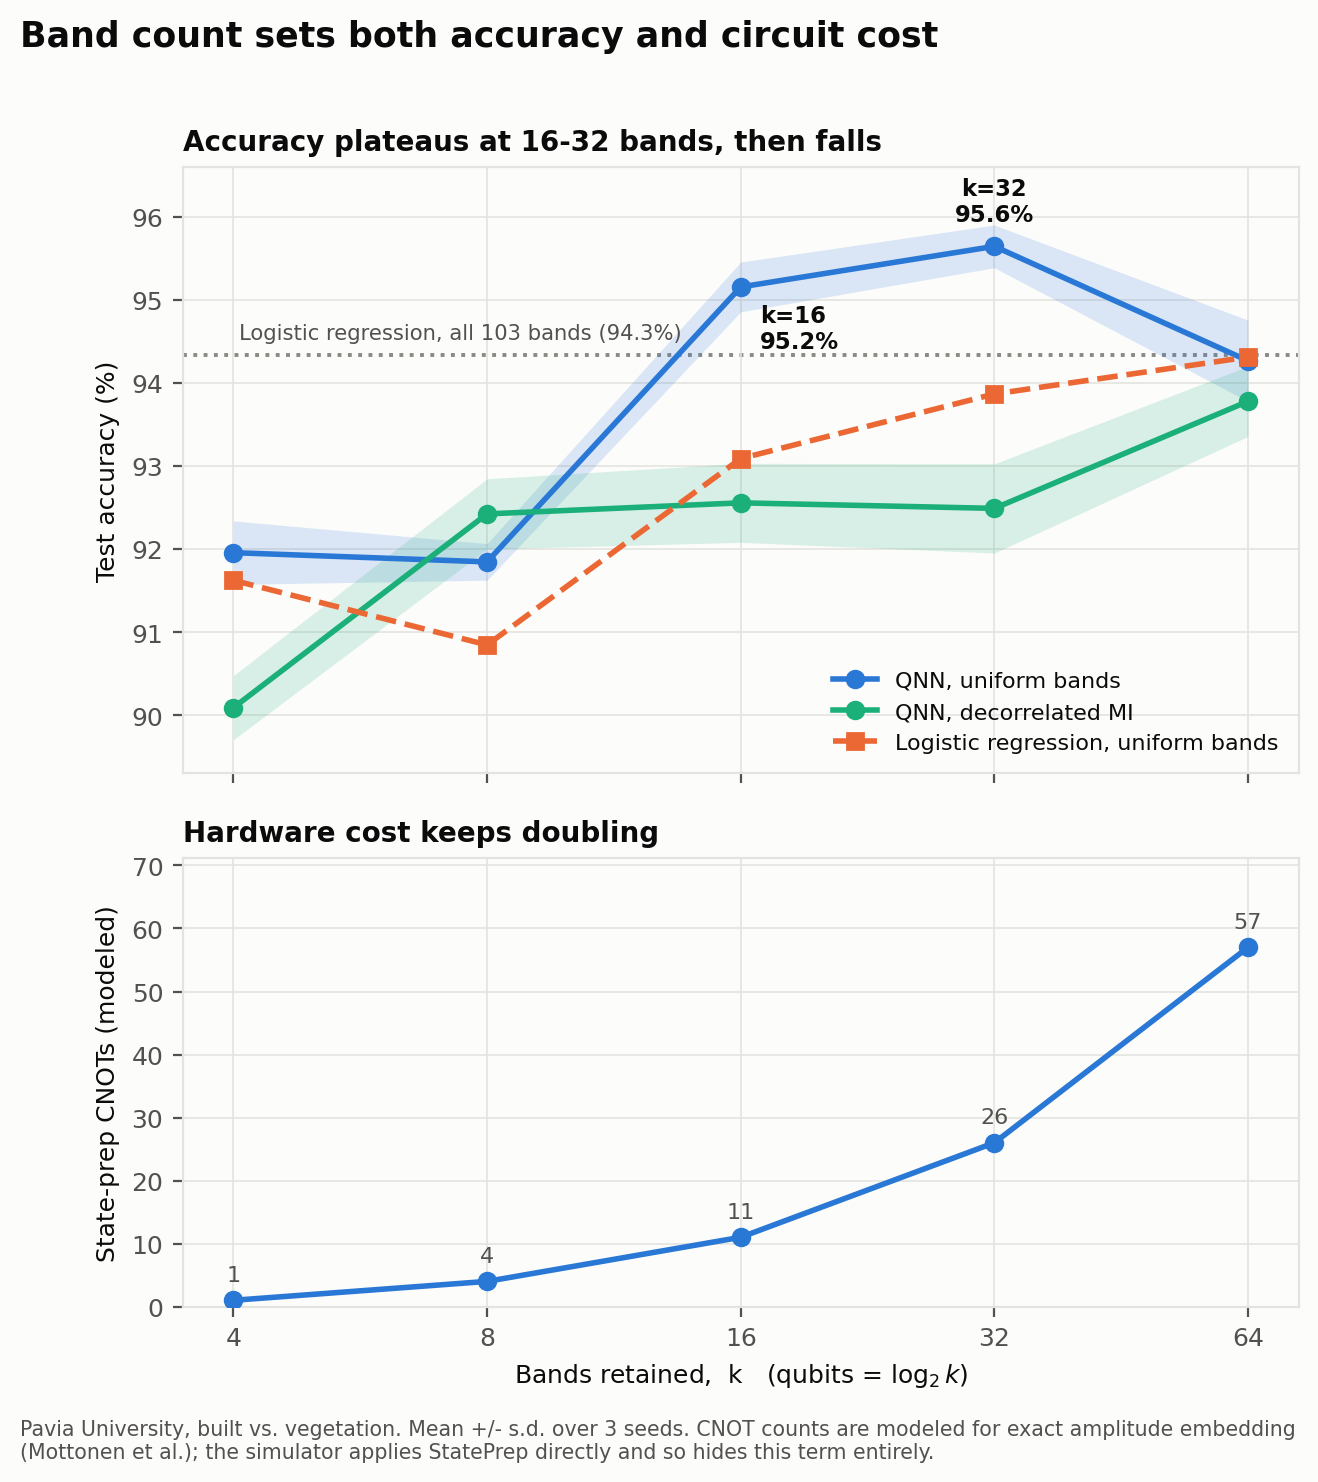
\includegraphics[width=\linewidth]{fig_scaling.png}
\end{center}

\vspace{5mm}
Accuracy peaks at 32 bands (95.6\%) and falls by 64. Moving from 16 to 64 bands
loses 0.9 percentage points while costing five times the state-preparation
CNOTs, because exact amplitude embedding scales as $O(2^{n})$. Uniformly spaced
bands beat supervised mutual-information selection at every $k \geq 16$~---
useful, since a fixed multispectral sensor supplies even spacing for free. The
quantum model's margin over logistic regression is 2.1 points at $k = 16$, and
gone by 64.

\columnbreak

%%% ------------------------------------------------------------- column 3 --
\sheadtop{Why inference is what costs}

Estimating a quantum expectation requires repeated measurement. The same pixel
through the same circuit returns a different answer each time, converging on the
exact value as $1/\sqrt{N}$~--- four times the shots buys twice the precision.
Built natively in both frameworks, PennyLane and Qiskit agree analytically to
$5\times10^{-16}$; what differs between runs is sampling, which both share.
Certainty is purchasable, and that is what makes inference, not training, the
recurring cost. \textbf{See the monitor.}

\vspace{22mm}
% -- bottom line: set apart by weight and space, deliberately not boxed ----
{\blsize\bfseries\color{ink}
Band selection, not qubit count, is the first-order cost variable for quantum
machine learning on satellite imagery.\par}
\vspace{22mm}

\shead{What this does not show}

This is single-date per-pixel classification on a proxy scene~--- not
bi-temporal change detection over a real data centre. All results are noiseless
simulation; nothing ran on quantum hardware. CNOT counts are modelled for exact
amplitude embedding rather than measured, because the simulator applies state
preparation in a single operation and hides the term entirely. Three seeds per
point.
\gap
The classical baseline here is logistic regression. A geospatial foundation
model~--- Scale-MAE, arXiv:2212.14532~--- is the stronger comparison, and is the
next benchmark rather than a demonstrated result.
\gap
One arithmetic note: the source paper's per-sample cost inverts its own
spreadsheet's units, which compute samples per minute~--- implying 28\,s and
roughly \$45 per sample rather than the stated 2\,min 13\,s.

\vspace{20mm}
\begin{minipage}[b]{0.60\linewidth}
{\finesize\color{ink2}
Sources: Rybotycki, Gupta \& Gawron, arXiv:2503.08962v3 \textperiodcentered{}
Zenodo 14784888 \textperiodcentered{} Pavia University (ROSIS)
\textperiodcentered{} Krawec, FAS \textperiodcentered{} EPRI.\\[4mm]
Code: github.com/deepeshmode/quantumml\\[4mm]
With thanks to Siwei Qiu.\par}
\end{minipage}\hfill
\begin{minipage}[b]{0.34\linewidth}
\raggedleft
\includegraphics[width=0.9\linewidth]{qr_repo.png}
\end{minipage}

\end{multicols}
\end{document}
